% Boilerplate from: https://github.com/jdavis/latex-homework-template/blob/master/homework.tex
\documentclass[table]{article}
\usepackage[table]{xcolor}
\usepackage{amssymb}
\usepackage{fancyhdr}
\usepackage{extramarks}
\usepackage{amsmath}
\usepackage{amsthm}
\usepackage{amsfonts}
\usepackage{tikz}
\usepackage{graphicx}
\usepackage{enumitem}
\usepackage{logicproof}

\topmargin=-0.45in
\evensidemargin=0in
\oddsidemargin=0in
\textwidth=6.5in
\textheight=9.0in
\headsep=0.25in

\linespread{1.1}
\pagestyle{fancy}
\lhead{\hmwkAuthorName}
\chead{\hmwkTitle}
\rhead{}
\cfoot{\thepage}

\renewcommand\headrulewidth{0.4pt}
\renewcommand\footrulewidth{0.4pt}

\setcounter{secnumdepth}{0}

\newcommand{\hmwkTitle}{Final Exam}
\newcommand{\hmwkDueDate}{23 July 2020}
\newcommand{\hmwkClass}{Discrete Structures}
\newcommand{\hmwkClassTime}{Section 201}
\newcommand{\hmwkClassInstructor}{Professor Jensen}
\newcommand{\hmwkAuthorName}{\textbf{Brian Ton}}

\title{
    \vspace{2in}
    \textmd{\textbf{\hmwkClass:\ \hmwkTitle}}\\
    \normalsize\vspace{0.1in}\small{Due\ on\ \hmwkDueDate}\\
    \vspace{0.1in}\large{\textit{\hmwkClassInstructor\ \hmwkClassTime}}
    \vspace{3in}
}

\author{\hmwkAuthorName}
\date{}

\newcolumntype{g}{>{\columncolor{yellow!20}}c}

\begin{document}
\maketitle
\pagebreak
\section{Problem 1}
Write the contrapositive of ``If $a \nmid b$ and $a \mid c$, then $a \nmid (b + c)$.''
\subsection{Solution}
If $a \mid (b+c)$ then $a \mid b$ or $a \nmid c$.
\subsubsection{Explanation}
Let $p$ be the statement $a \nmid b$, $q$ be the statement $a \mid c$, and $r$ be the statement $a \nmid (b+c)$.\\
Symbolically, the original statement can thus be written as $(p \land q) \rightarrow r$. The contrapositive would then be $\neg r \rightarrow \neg (p \land q)$ which by De Morgan's law would be $\neg r \rightarrow (\neg p \lor \neg q)$, which in English would be ``If $a \mid (b+c)$ then $a \mid b$ or $a \nmid c$.''
\section{Problem 2}
Consider the function $f$ from set $X$ to set $Y$. Write the negation of the following definition for $f$ to
be one-to-one.\\
$\forall x_1, x_2 \in X$, if $f(x_1)=f(x_2)$, then $x_1=x_2$.
\subsection{Solution}
$\exists x_1, x_2 \in X$, such that $f(x_1)=f(x_2)$ and $x_1 \neq x_2$.
\subsubsection{Explanation}
Writing the original statement in full symbolic form, it becomes $\forall x_1, x_2 \in X, (f(x_1)=f(x_2) \rightarrow x_1=x_2)$.
Note that we use logical equivalences to find the negation.\\
\begin{align*}
\neg \forall x_1, x_2 \in X, (f(x_1)=f(x_2) \rightarrow x_1=x_2)
&\equiv \exists x_1, x_2 \in X, \neg (f(x_1)=f(x_2) \rightarrow x_1=x_2) && \text{(De Morgan's Law)}\\
&\equiv \exists x_1, x_2 \in X, (f(x_1)=f(x_2) \land \neg (x_1=x_2)) && \text{$(\neg (p \rightarrow q) \equiv p \land \neg q)$}\\
&\equiv \exists x_1, x_2 \in X, (f(x_1)=f(x_2) \land (x_1 \neq x_2))\\
\end{align*}
Putting this back to match the original statement, $\exists x_1, x_2 \in X$, such that $f(x_1)=f(x_2)$ and $x_1 \neq x_2$.
\section{Problem 3}
$\sqrt{3}$ is irrational. Use proof by contradiction to prove the statement ``$4\sqrt{3} - 7$ is irrational.''
\subsection{Solution}
\textbf{Proof By Contradiction}
Assume $4\sqrt{3} - 7$ is rational.\\
By definition of a rational number, $4\sqrt{3} - 7 = \frac{p}{q}$ for some integers $p$ and $q$. Hence, we can write $4\sqrt{3} = \frac{p}{q} + 7$. This would mean that $4\sqrt{3} = \frac{p+7q}{q}$. Then, $\sqrt{3} = \frac{p+7q}{4q}$. Note that by closure of the integers under addition and multiplication, $p+7q$ and $4q$ is an integer. However, this would mean that $\sqrt{3}$ can be written as the ratio of two integers, which would mean that it is rational by the definition of a rational number. This is a contradiction, by the given information. Hence, the initial assumption that $4\sqrt{3} - 7$ is rational is false, meaning that $4\sqrt{3} - 7$ is irrational.
\section{Problem 4}
A sequence $m_1, m_2, m_3, ...$ is defined by letting $m_1 = 1$ and $m_k = 2m_{k-1} + 1$, for all integers $k \geq 2$. Use induction to show that $m_n = 2^n - 1$, for all integers $n \geq 1$.
\subsection{Solution}
\textbf{Proof By Induction}\\
\textbf{Base Case:} Show that $m_1 = 2^n-1$ for $n \geq 1$. By definition, $m_1 = 1$. Note that for $n=1$, $2^1-1=2-1=1=m_1$. This completes the basis step.\\
\textbf{Inductive Hypothesis:} Assume that $m_k = 2^k-1$ for some fixed integer $k \geq 1$.\\
\textbf{Inductive Step:} By definition of the sequence:
\begin{align*}
m_{k+1}
&= 2m_k+1\\
&= 2(2^k-1)+1 && \text{(Inductive Hypothesis)}\\
&= 2^{k+1} - 2 + 1\\
&= 2^{k+1} - 1
\end{align*}
Hence, by induction, $m_n = 2^n-1$.
\section{Problem 5}
\begin{enumerate}[nosep,label=\alph*)]
\item State the Well-Ordering Principle for the integers.
\item Does the set of all positive real numbers have a least element? If not, explain why the well-ordering principle is not violated.
\item Does the set of all nonnegative integers $n$ such that $n^2 < n$ have a least element? If not, explain why the well-ordering principle is not violated.
\end{enumerate}
\subsection{Solution}
\begin{enumerate}[nosep,label=\alph*)]
\item Every nonempty set of nonnegative integers has a least element.
\item No, the set of positive real numbers does not have a least element. For instance, let $x$ be the smallest positive real number. However, note that $\frac{x}{2}$ is a positive real number and $\frac{x}{2} < x$, which means that there can be no smallest positive real number. This does not violate the well-ordering property, as the property's definition states that it applies to integers, not to real numbers.
\item There does not exist a least element in the set of all nonnegative integers $n$ such that $n^2 < n$. This is because $n^2<n$ only for real numbers $0 < n < 1$. Hence, the set will be empty, since there are no integers between $0$ and $1$. This does not violate the well-ordering property since the well ordering property only applies to nonempty sets.
\end{enumerate}
\section{Problem 6}
Define a binary relation $R$ on $A = \{0, 1, 2, 3\}$ as $R = \{(0,0), (0,1), (1,1), (1,2), (2,3), (3,3)\}$.
\begin{enumerate}[nosep,label=\alph*)]
\item Draw the directed graph.
\item Is R reflexive? Answer Yes or No. If not, provide a counterexample.
\item Is R symmetric? Answer Yes or No. If not, provide a counterexample.
\item Is R transitive? Answer Yes or No. If not, provide a counterexample.
\item Is R an equivalence relation? Answer Yes or No. Explain.
\end{enumerate}
\subsection{Solution}
\subsubsection{Part A}
\begin{figure}[h!]
	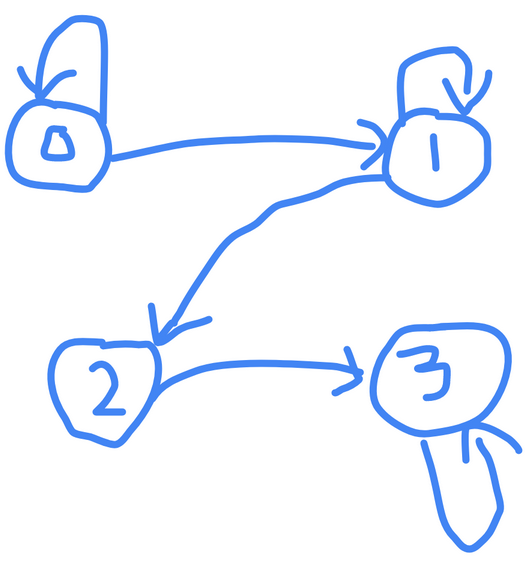
\includegraphics[scale=.3]{images/Prob6a.png}
\end{figure}
\subsubsection{Part B}
$R$ is not reflexive. This is because $(2, 2) \not\in R$.
\subsubsection{Part C}
$R$ is not symmetric. This is because while $(2, 3) \in R$, $(3, 2) \not\in R$.
\subsubsection{Part D}
$R$ is not transitive. This is because while $(0, 1) \in R$ and $(1, 2) \in R$, $(0, 2) \not\in R$.
\subsubsection{Part E}
Since $R$ is not reflexive, symmetric, and transitive, $R$ is not an equivalence relation.
\section{Problem 7}
Let $A = \{a, b, c, d\}$ and $B = \{1, 2, 3\}$. Answer the following questions without listing the elements. Show your work.
\begin{enumerate}[nosep,label=\alph*)]
\item How many elements are in the set $A \times B$?
\item How many binary relations are there from $A$ to $B$
\item How many functions are there from $A$ to $B$?
\item How many one-to-one functions are there from $A$ to $B$?
\item How many onto functions are there from $A$ to $B$?
\end{enumerate}
\subsection{Solution}
\subsubsection{Part A}
Note that since each element in $A$ must be in an ordered pair with each element in $B$, $|A \times B| = |A| \cdot |B|$. Hence, there will be $4 \cdot 3 = 12$ elements in $A \times B$.
\subsubsection{Part B}
Since a binary relation is a subset of $A \times B$ by definition, the number of binary relations would thus be $|\mathcal{P}(A \times B)|$, since we want the number of subsets of $A \times B$, which by definition would be the power set of $A \times B$. By a known fact, $|\mathcal{P}(A)|=2^{|A|}$. Since $|A \times B| = 12$ by part A, $|\mathcal{P}(A \times B)|=2^{12}=4096$. Hence, there are $4096$ binary relations from $A$ to $B$.
\subsubsection{Part C}
Since every element in $A$ has $|B|$ number of choices to match to, and each choice leads to a unique function, in general, the number of functions from $A$ to $B$ is $|B|^{|A|}$. This reasoning is equivalent to noticing that every element in $A$ is in $|B|$ ordered pairs in $A \times B$. By definition of a function, each element in $A$ must map to exactly 1 element in $B$. Then, the number of choices of ordered pairs per element in $A$ is $|B|$, which means that the total number of functions is $|B| \cdot |B| \cdot ...$, $|A|$ times. This means that the number of functions is then $|B|^{|A|}$. Hence, there are $3^4=81$ possible functions from $A$ to $B$.
\subsubsection{Part D}
Notice that there are $3$ elements in $B$ and $4$ elements in $A$. In order for a function from $A$ to $B$ to be one-to-one, each element in $B$ must map to at most $1$ element in $A$. By the pigeonhole principle, this cannot be true. Hence, there are $0$ one-to-one functions from $A$ to $B$.
\subsubsection{Part E}
For such an onto function to exist, $1$ element from $B$ must map to exactly $2$ elements in $A$, with the other two elements in $A$ mapping to different elements in $B$. Combinatorially, there are $3 \choose 1$ elements to choose $1$ element from a set of $3$ elements, and $4 \choose 2$ ways to choose $2$ elements from a set of $4$ elements. Hence, there are ${3 \choose 1} \cdot {4 \choose 2}=18$ ways to have $2$ elements from a set of $4$ map to $1$ element in a set of $3$. There are then $2$ ways to map the remaining $2$ elements in $A$ to a unique element in $B$. Thus, by the multiplication principle, there are $18 \cdot 2 = 36$ onto functions from $A$ to $B$.
\section{Problem 8}
\begin{enumerate}[nosep,label=\alph*)]
\item \textit{True} or \textit{False}. The set of rational numbers is countable.
\item \textit{True} or \textit{False}. The set of real numbers is uncountable.
\end{enumerate}
\subsection{Solution}
\begin{enumerate}[nosep,label=\alph*)]
\item True
\item True
\end{enumerate}
\section{Problem 9}
Consider a class of ten students.
\begin{enumerate}[nosep,label=\alph*)]
\item In how many ways can the teacher give three different prizes to three of her ten students?
\item In how many ways can a team of three players be selected from the ten students?
\end{enumerate}
\subsection{Solution}
\begin{enumerate}[nosep,label=\alph*)]
\item Since order matters in this case (because each prize is different) and we are looking for the number of ways to assign $3$ different people (note that it is implied that a student cannot be a repeat winner since there must be $3$ students that win and only $3$ prizes are given out) to these $3$ different prizes, permutations should be used to count the number of possibilities. Hence, there are $_{10}P_3 = \frac{10!}{(10-3)!}=720$ ways to do this. An equivalent way of looking at this is to notice that there are $10$ students that the teacher can choose for the first prize, $9$ for the second, and $8$ for the third. By the multiplication principle, there are $10 \cdot 9 \cdot 8 = 720$ ways, then, to give out the prizes.
\item Since order does not matter, and a student cannot take up more than 1 slot in a team, combinations should be used to determine the number of ways to select the teams. There are ${10 \choose 3} = \frac{10!}{3!(10-7)!} = 120$ ways to select a team of $3$ players from a group of $10$.
\end{enumerate}
\section{Problem 10}
A new, simple test has been developed to detect a particular type of cancer. The test must be evaluated before it is used. A medical researcher selects a random sample of $1,000$ adults and finds (by other means) that $2\%$ have this type of cancer. Each of the $1,000$ adults is given the test, and it is found that the test indicates cancer in $98\%$ of those who have it and in $1\%$ of those who do not. Based on these results, what is the probability of a randomly chosen person not having cancer given that the test indicates cancer? (That is, what is the probability of the test giving a false positive result?)
\subsection{Solution}
Let $E$ be the event where the person has a positive test result (i.e. the test indicates cancer) and $F$ be the event where the person does not have cancer. The probability that the person does not have cancer given a positive test can be written as $P(F|E)$. From the problem, it is known that $P(F)=98\%=0.98$, $P(E|F)=1\%=0.01$, and $P(E|\overline{F})=98\%=.98$. From this, we can also conclude that $P(\overline{F})=2\%=.02$. By Bayes' Theorem, $P(F|E) = \frac{P(E|F)P(F)}{P(E|F)P(F)+P(E|\overline{F})P(\overline{F})}=\frac{.01 \cdot .98}{.01 \cdot .98 + .02 \cdot .98}=\frac{.01 \cdot .98}{.98(.01 + .02)}=\frac{.01}{.03}=\frac{1}{3} \approx 33.3\%$.
\section{Problem 11}
There are $23$ dachshunds and $22$ dog beds. Each dachshund goes to a dog bed. Does each dachshund have a bed to himself? \textit{Yes} or \textit{No}. What is the name of the principle you applied?
\subsection{Solution}
Since there are more dogs than dog beds (i.e. places where the dogs can go), by the pigeonhole principle, there is no way to arrange the dogs such that the dogs each have a bed to themselves.
\section{Problem 12}
Is it possible to have a graph with $13$ vertices each of degree $7$? Answer \textit{Yes} or \textit{No}.
\subsection{Solution}
\textbf{No}\\
Notice that by the definition of this graph $G(V, E)$, $\sum_{v \in V}^{} deg(v) = 13 \cdot 7 = 91$. By the Handshaking Theorem, the sum of the degree of each vertex must be $2|E|$, meaning that the sum of the degree of each vertex must be an even number. However, since $91$ is not even and thus the sum of the degree of each vertex is not even, the graph cannot exist, since it would contradict the Handshaking Theorem.
\section{Problem 13}
For each statement answer \textit{Always}, \textit{Sometimes}, or \textit{Never}.
\begin{enumerate}[nosep,label=\alph*)]
\item A connected graph with five vertices of degrees $2$, $4$, $1$, $2$, and $3$ has a Euler circuit.
\item A connected graph with five vertices of degrees $2$, $4$, $2$, $4$, and $2$ has a Euler circuit.
\item A graph with five vertices of degrees $2$, $4$, $2$, $4$, and $2$ has a Euler circuit.
\end{enumerate}
\subsection{Solution}
\begin{enumerate}[nosep,label=\alph*)]
\item Never. By Theorem $1$ in Section $10.5$, a connected multigraph of at least two vertices has an Euler circuit iff each of its vertices has an even degree. Here, note that the graph is a connected one in its definition. However, note that the graph has vertices of degree $1$ and $3$, both of which are not even. Hence, by Theorem $1$, there cannot exist an Euler circuit.
\item Always. By Theorem $1$ in Section $10.5$, a connected multigraph of at least two vertices has an Euler circuit iff each of its vertices has an even degree. Here, note that the graph is connected by its definition. Additionally, note that the graph has vertices with degrees being all even numbers. Hence, by Theorem $1$, there always exists an Euler circuit.
\item Sometimes. By Theorem $1$ in Section $10.5$, a connected multigraph of at least two vertices has an Euler circuit iff each of its vertices has an even degree. Here, note that the graph has vertices with degrees being all even numbers. However, such a graph is not necessarily a connected one. If it is connected, by Theorem $1$, then there would exist an Euler circuit. However, if it is not connected, then there does not exist an Euler circuit. Hence, the graph will only sometimes have an Euler circuit.
\end{enumerate}
\end{document}